			\documentclass{article}
			\usepackage[margin=1.25in]{geometry}
			\usepackage{graphicx}
			\usepackage{listings}
			\usepackage{titlepic}
			\usepackage{afterpage}
\usepackage{textcomp}
			\usepackage{float}
\usepackage[figuresleft]{rotating}
			\usepackage{hyperref}
\usepackage{xcolor}
			\newcommand\tab[1][1cm]{\hspace*{#1}}
			\usepackage{multicol}
			\renewcommand{\labelenumii}{\theenumii}
			\newcommand{\quotes}[1]{``#1''}
			\renewcommand{\theenumii}{\theenumi.\arabic{enumii}.}
			
			\begin{document}
			\title{
\includegraphics[scale = .6]{uom.png}
				\linebreak 
				\textbf{CPS2000 - Compiler Theory \& Practise}\linebreak\linebreak
				\textbf{Assignment Part 2}\linebreak\linebreak
				\large{B.Sc Computer Science}
				\date{}
				\author{Jacques Vella Critien - 97500L}}
				
				\begin{titlepage}
					\maketitle
					\thispagestyle{empty}
				\end{titlepage}
				
				\tableofcontents
				\newpage
				
				\section{Task1: Extending SmallLang}
				
				For the first task of this part of the assignment, we were required to extend SmallLang into SmallLangV2 by adding some other features. These features include adding support for the primitive type \quotes{char} and for arrays which hold a series of elements of the same type in contiguous memory. It was required to let array values uninitialised by default but an implementation for initialisation for values was also required. Moreover, formal parameters had to be changed in order to support both the \quotes{char} type and the arrays as types. In order to implement this, as can be seen below, EBNF rules had to be added and some were changed.
				
				\subsection{Solution}
				
				The rules below show the new and changed rules. The other rules which were present in SmallLang and not included in the below set, have not changed.
				
				\begin{lstlisting}[backgroundcolor=\color{lightgray},basicstyle=\small,upquote=true]
				
  <ArraySizeIndex> 	::= '[' <Expression> ']'
  
  <ArrayIdentifier> 	::= <Identifier> <ArraySizeIndex>
  
  <ArrayValue> 		::= '{' <Expression> { ',' <Expression> } '}'
  
  <VariableDecl> ::= <Identifier> ':' (<Type>|<Auto>) '=' <Expression> 
  
  <ArrayDecl> 	::=  <ArrayIdentifier>`:' <Type> ['=' <ArrayValue>] 
  
  <FormalParam> 	::= <Identifier> [ '[' ']' ] : <Type>
  
  <AbstractIdentifier>	::= <Identifier> | <ArrayIdentifier>
  
  <Assignment>	::= <AbstractIdentifier> `=' <Expression>
  
  <Decl> 		::= 'let' (<VariableDecl> | <ArrayDecl>)
  
  <CharLiteral>  	::= '\'' <Letter> '\''
  
  <Literal> 		::= <BooleanLiteral>
  			 |  <IntegerLiteral>
  			 |  <FloatLiteral>
  			 |  <CharLiteral>
  					
  <Factor> 		::= <Literal>
  			 |  <AbstractIdentifier>
  			 |  <FunctionCall>
  			 |  <SubExpression>
  			 |  <Unary>
  
  <Statement> 		::= <Decl> ';'
  			|   <Assignment ';'
  			|   <PrintStatement> ';'
  			|   <IfStatement> 
  			|   <ForStatement> 
  			|   <WhileStatement> 
  			|   <RtrnStatement> ';'
  			|   <FunctionDecl>
  			|   <Block>
  
  
  	
				  
				\end{lstlisting}
				
				
				\subsubsection{\textless ArraySizeIndex\textgreater}
				
				This rule represents the size of the array in the case of a declaration while it represents the index to assign in an assignment. It consists of an expression in the middle of square brackets. The expression would then be checked by the semantic analyser to make sure that it is of type int.
				
				\subsubsection{\textless ArrayIdentifier\textgreater}
				
				This rule represents an array identifier and it consists of an identifier followed by the above rule, which represents the size or the index.
				
				\subsubsection{\textless ArrayValue\textgreater}
				
				This rule represents the value to set to the array on declaration. This consists of an expression or more inside curly brackets.
				
				\subsubsection{\textless VariableDecl\textgreater}
				
				This rule represents a variable declaration for an array. I updated it by removing the 'let' from the start and starting with an <Identifier> node before a semi colon and a type which can also be auto. Finally, it remains the same by expecting an equal sign and an expression
				
				\subsubsection{\textless ArrayDecl\textgreater}
				
				This rule represents the declaration for an array. It starts with an \textless ArrayIdentifier\textgreater{} node explained above before a semi colon and a type. As can be seen in the figure above, an equals sign and an \textless ArrayValue\textgreater{} node are optional because arrays can be initialised or uninitailised in declarations.
				
				
				\subsubsection{\textless Decl\textgreater}
				
				Similarly, this new rule just represents either a variable declaration or an array declaration node by first expecting a let and then, either type of declaration.
				
								\subsubsection{\textless Assignment\textgreater}
				
								This rule is an updated version of the \textless Assignment\textgreater{} rule from part 1 of this assignment. As can be seen, this rule now accepts an ASTAbstractIdentifier which includes both ASTArrayIdentifier and ASTIdentifier rather than just ASTIdentifier.
				
				
				\subsubsection{\textless FormalParam\textgreater}
				
				This rule is an updated version of the \textless FormalParam\textgreater{} rule from part 1 of this assignment. As can be seen, optional empty square brackets are possible after the identifier which indicates an array as a formal parameter. Despite it is listed as an identifier, the actual code in the parser looks for a trailing `[` and if it is found an ASTArrayIdentifier node is returned and not an ASTIdentifier.
				
				\subsubsection{\textless AbstractIdentifier\textgreater}
				
				This new rule just represents either a normal identifier or an array identifier rule.
								
				
				\subsubsection{\textless CharLiteral\textgreater}
				
				This new rule was added to represent a character literal and it consists of a \textless Letter\textgreater{} rule in between two apostrophes.
				
				\subsubsection{\textless Literal\textgreater}
				
				This rule represents a literal and was updated to be able to also represent a \textless CharLiteral\textgreater {} rule.
				
				\subsubsection{\textless Factor\textgreater}
				
				This rule was updated to be able to represent an \textless AbstractIdentifier\textgreater{} rule instead of an \textless Identifier\textgreater{} rule to be able to also represent an \textless ArrayIdentifier\textgreater{} rule.
				
				\subsubsection{\textless Statement\textgreater}
				
				This rule was updated to be able to represent a \textless Decl\textgreater{} rule instead of an \textless VariableDecl\textgreater{} rule to be able to also represent an \textless ArrayDecl\textgreater{} rule.
				
				
				\section{Task1: SmallLangV2 Lexer and Parser}
				
				The second task required was to implement the necessary changes for the lexer and parser in order to process the input program containing the new features, namely the character literal and arrays. In order to perform this, I started off by extending the DFA (Deterministic Finite Automaton) to be able to split the inputs into correct tokens. Moreover, as will be explained below, the three tables which are the \quotes{Classifier Table}, the \quotes{Type Token Table} and the \quotes{Transition table} were also changed. Finally, for the parser, new nodes were created and the Parser class was updated. 
				
				\subsection{Deterministic Finite Automaton}
				
				The figure below shows the added items to the automaton in part 1 so that the new features can be applied. As can be easily seen, State S28 represents a `[' token, State S29 represents the `]' token and S32 represents a character literal token, whose lexeme is in the form of `\textless character\textgreater'. \textbf{Once again, it is important to note that for each state, any other character inserted which are not visible in the paths going out from that state ALL lead to an absorbing bad state. This is not included in the diagram just to keep the diagram clear.}
				
				\begin{center}
					\begin{figure}[H]
			 			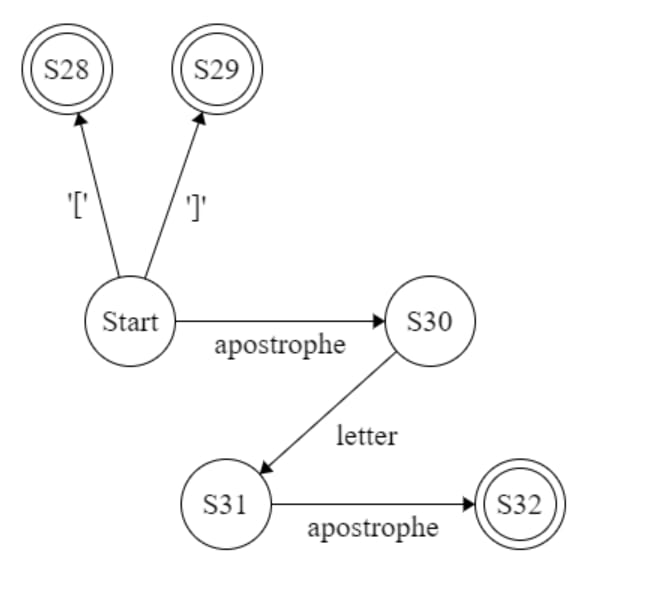
\includegraphics[width=0.6\textwidth]{part2automaton.jpeg}
			 			\centering
			  			\caption{Deterministic finite automaton additions}
			  			\label{fig:automaton}
					\end{figure}
				\end{center}
				

			\subsection{Tables}
			\subsubsection{Classifier Table}
			
			This table which relates the specific characters of input to the classifiers was updated in order to support the three new classifiers or categories. The new classifiers can be seen below and these were added to the the Classifier table created for part 1 of the assignment. The top row shows the character inputted and the bottom row shows the related classifier.
			
			 \begin{center}
					\begin{figure}[H]
			 			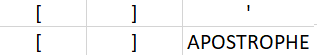
\includegraphics[width=0.4\textwidth]{ctpart2.png}
			 			\centering
			  			\caption{Classifier Table additions}
			  			\label{fig:cttable}
					\end{figure}
				\end{center}
				
				\subsubsection{Type Token Table}
			
			This table which relates states to the classifiers was updated in order to support the five new states. The new states can be seen below and these were added to the the Type Token table created for part 1 of the assignment. The top row shows the state and the bottom row shows the related classifier.
			
			 \begin{center}
					\begin{figure}[H]
			 			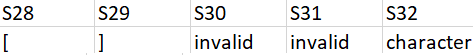
\includegraphics[width=0.6\textwidth]{ttpart2.png}
			 			\centering
			  			\caption{Type Token Table additions}
			  			\label{fig:tttable}
					\end{figure}
				\end{center}
				
				
				\subsubsection{Transition Table}
			
			This table which represents transitions from one state to another state when given a classifier, was updated in order to add the three new classifiers and the five new states. The transitions involving the new classifiers and states can be seen below marked in red. This was done to be able to distinguish them from previously created transitions for part 1 of the assignment. The columns represent the classifiers while the rows represent the states.
			
			 \begin{sidewaysfigure}
			 			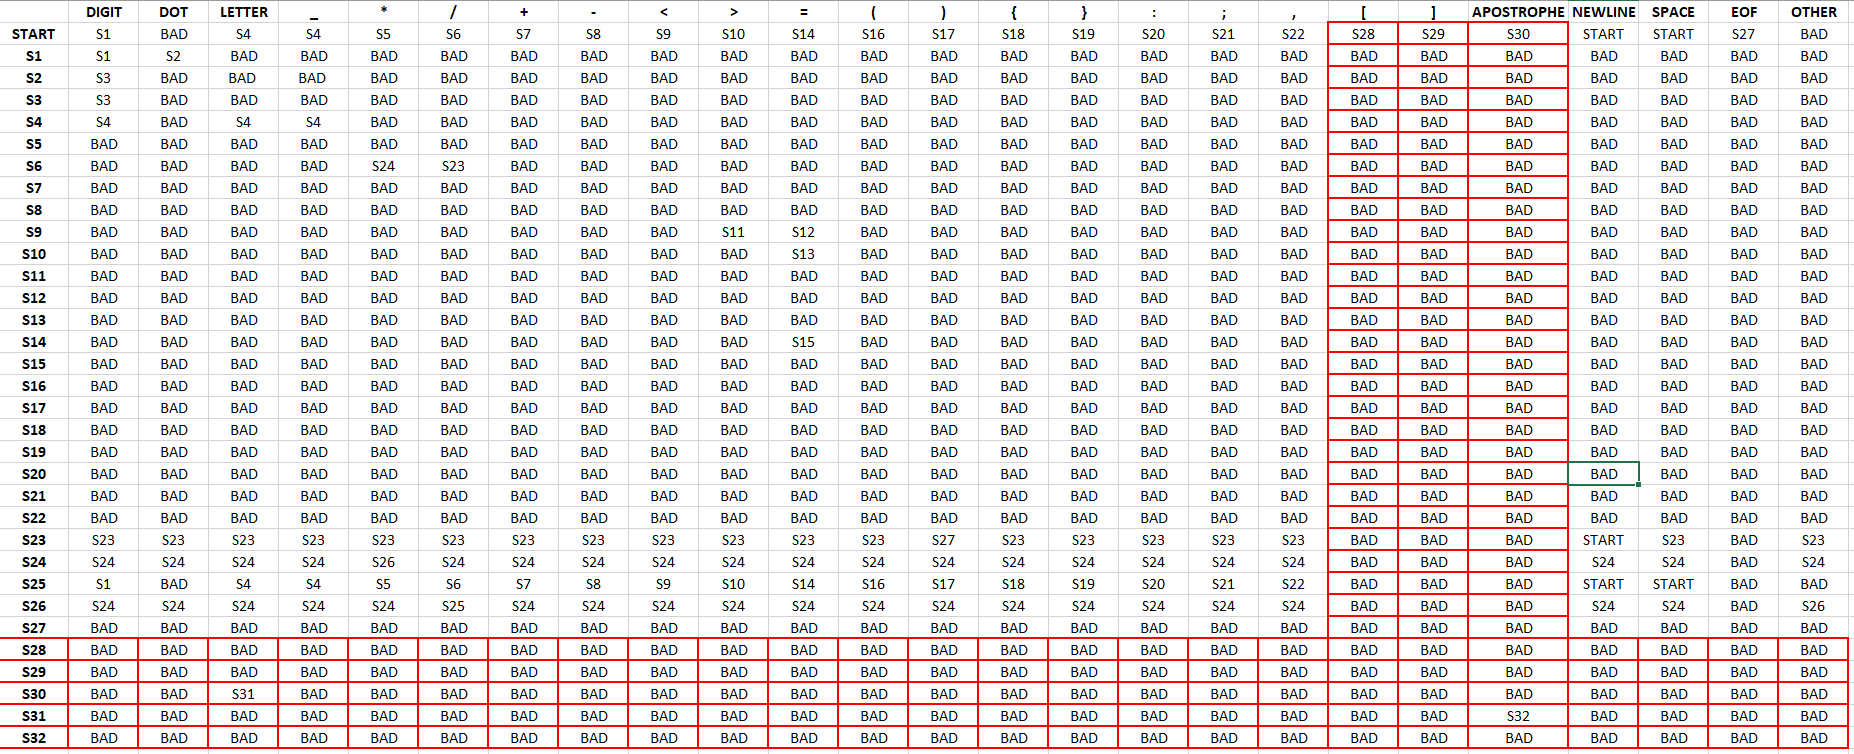
\includegraphics[width=\textwidth]{txpart2.png}
			 			\centering
			  			\caption{Transition Table additions}
			  			\label{fig:txtable}
				\end{sidewaysfigure}
			
			\pagebreak
			
			\subsection{Lexer Solution}
			
			This section highlights and explains the difference and additions made in the code to support these new features in relation to the \textbf{lexer}.
			
			\subsubsection{TypeToken.java}
					
					This enum class which holds the different types of tokens was updated to include the following:
					\begin{itemize}
						\item SQUARE\_OPEN
						\item SQUARE\_CLOSE
						\item CHARACTER\_LITERAL
					\end{itemize}
				
				\subsubsection{Category.java}
					
					This enum class which holds the different types of categories or classifiers was updated to include these three new classifiers:
					\begin{itemize}
						\item SQUARE\_OPEN
						\item SQUARE\_CLOSE
    						\item APOSTROPHE
					\end{itemize}
					
				      \subsubsection{State.java}
					
					This enum class which holds the different types of states was updated to include these 5 new states:
					\begin{itemize}
						\item S28
						\item S29
    						\item S30
    						\item S31
    						\item S32
					\end{itemize}
					
					\subsubsection{Keyword.java}
					
					This class which extends the Token class and in which all the keywords in the SmallLangV2 syntax are declared was updated and a new keyword to represent the char primitive was created and defined with the name CHAR.
					
					\subsubsection{Lexer.java}
					
					This class which contains all the methods needed from the parser to obtain the next token was updated to be able to handle the new features. Below contains all the list of methods that were changed and how:
					
					\begin{enumerate}
					\item \textbf{setTransitionTable()}: This function which populates the transition table hashmap was updated by adding the new transitions involved with the new classifiers and states. Basically, all the added transitions are the ones marked in red in the figure found in section 2.2.3
					\item \textbf{setAcceptableStates()}: This function which populates the acceptable states hashmap was updated to include set states S28, S29 and S32 as acceptable states. These states can be confirmed as being acceptable and final from the automaton on section 2.1 and the Type Token table in section 2.2.2.
						\item \textbf{charCat()}: This function which returns the category of a particular character was updated to support the three new tokens and categories which can be found in the classifier table in section 2.2.1
						\item \textbf{nextToken()}: This method which is called by the parser to give out the next token was only changed in the last part, that is the result reporting by adding a clause to check if it is a character literal and if so, the apostrophes are removed from the lexeme. This can be seen from the code snippet below.
					\begin{center}
					\begin{figure}[H]
			 			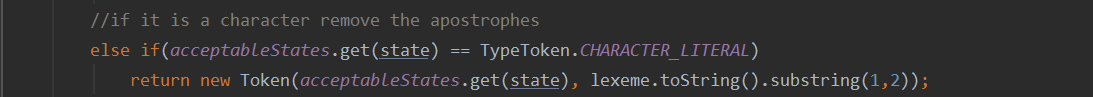
\includegraphics[width=0.8\textwidth]{lexerchange.png}
			 			\centering
			  			\caption{Change in nextToken() method}
			  			\label{fig:lexerchange}
					\end{figure}
				\end{center}
						
					\end{enumerate}
					

		\subsection{Parser Solution}
		
		This section highlights and explains the difference and additions made in the code to support these new features in relation to the \textbf{parser}.
		
		\subsubsection{ASTAbstractIdentifier.java}
					
					This is a class which extends the \textbf{ASTExpression} interface. This is extended by the \textbf{ASTIdentifier} and \textbf{ASTArrayIdentifier} classes. This class has the following 2 members: 
					\begin{enumerate}
					\item \textbf{name}: Its type is String and it is used to hold the variable name
					\item \textbf{type}: Its of type Type (enumeration) and it is used to hold the type of the identifier.
				
					\end{enumerate}
			In addition, this has getters for each member and a setter for the type to be used in case the identifier is of type auto so that it could be set to the expression's type as I will be explaining later.
			
			\begin{figure}[H]
					\centering
			 			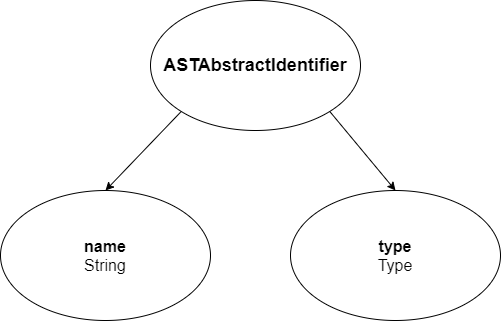
\includegraphics[width=0.55\textwidth]{astabstractid.png}
			  			\caption{ASTAbstractIdentifier node}
			  			\label{fig:astabstractid}
					\end{figure}
	
					
					
		\subsubsection{ASTIdentifier.java}
					
					This is a class which was created in part 1 of this assignment to represent an identifier. Now, it has been changed to extend the \textbf{ASTAbstractIdentifier} class and take up all of its member variables and methods which were explained in the above subsection highlighting the \textbf{ASTAbstractIdentifier} class.
					
					\begin{figure}[H]
					\centering
			 			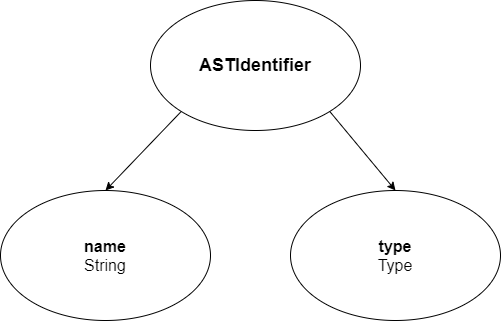
\includegraphics[width=0.55\textwidth]{astidentifier.png}
			  			\caption{ASTIdentifier node}
			  			\label{fig:astidentifier}
					\end{figure}
					
							\subsubsection{ASTArrayIdentifier.java}
					
					This is a class which extends the \textbf{ASTExpression} interface. This is extended by the \textbf{ASTIdentifier} and \textbf{ASTArrayIdentifier} classes. This class has the following 3 members: 
					\begin{enumerate}
					\item \textbf{name}: Its type is String and it is used to hold the variable name
					\item \textbf{sizeIndex}: Its of type ASTExpression and it is used to hold the size or index of the array identifier.
					\item \textbf{type}: Its of type Type (enumeration) and it is used to hold the type of the identifier.
				
					\end{enumerate}
			In addition, this has getters for each member, some of which are inherited from the ASTAbstractIdentifier class.
					
								\begin{figure}[H]
					\centering
			 			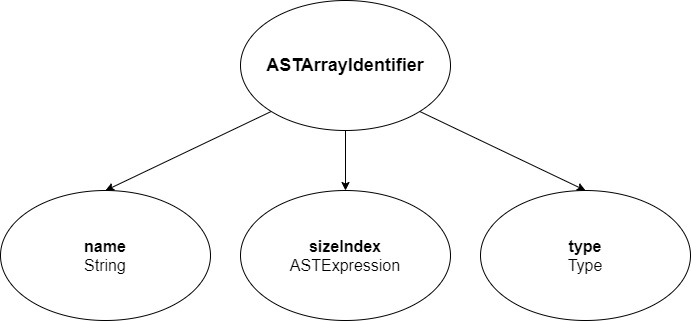
\includegraphics[width=0.55\textwidth]{astarrayidentifier.png}
			  			\caption{ASTArrayIdentifier node}
			  			\label{fig:astarrayidentifier}
					\end{figure}
					
							\subsubsection{ASTArrayValue.java}
					
					This is a class which extends the \textbf{ASTNode} interface. This was created to represent the value used to initialise an array, This class also has a member variable named values which is an arraylist of expressions of the type \textbf{ASTExpression}. In addition, this class also consists of constructors to create an object of this type,
					
								\begin{figure}[H]
					\centering
			 			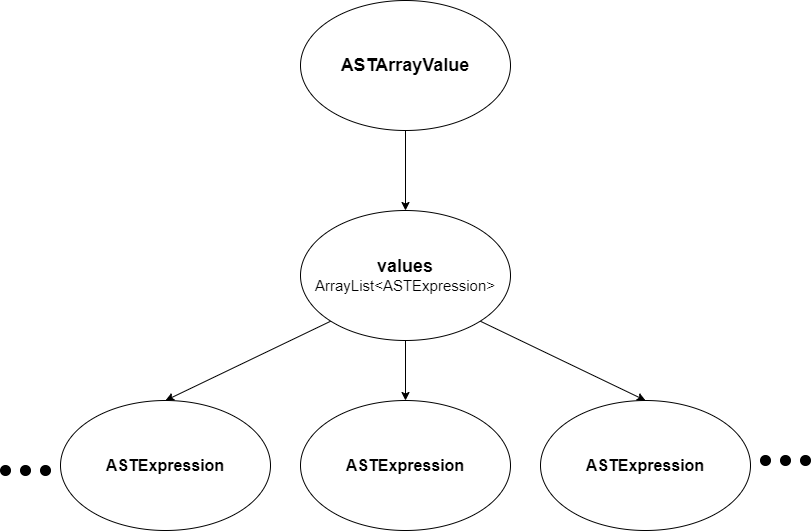
\includegraphics[width=0.55\textwidth]{astarrayvalue.png}
			  			\caption{ASTArrayValue node}
			  			\label{fig:astarrayvalue}
					\end{figure}					
					
										\subsubsection{ASTDecl.java}
					
					This is a class which extends the \textbf{ASTStatement} interface. This is extended by the \textbf{ASTVariableDecl} and \textbf{ASTArrayDecl} classes.
					
										\subsubsection{ASTVariableDecl.java}
					
					This is a class represents a variable declaration and was declared in part 1 of this assignment. The only change to this class was to make it extend the \textbf{ASTDecl} class.
					
					\subsubsection{ASTArrayDecl.java}
					
					This class was added to represent an array declaration. It extends the newly ASTDecl class and contains the following two member variables:
					
					\begin{enumerate}
					\item \textbf{values}: Its type is ASTArrayValue and it is used to hold the array values to be declared. This can be left empty if the array is declared but not initialised.
					\item \textbf{identifier}: Its of type ASTArrayIdentifier and it is used to identifier of the newly created array
				
					\end{enumerate}
			In addition, this also contains a constructor to create a new instance of this class.
			
							\begin{figure}[H]
					\centering
			 			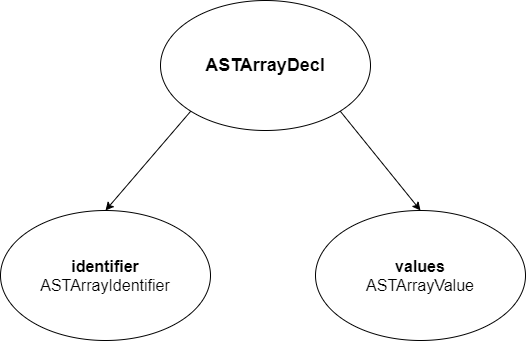
\includegraphics[width=0.4\textwidth]{arraydecl.png}
			  			\caption{ASTArrayDecl node}
			  			\label{fig:astarraydecl}
					\end{figure}
					
					
					\subsubsection{ASTAssignment.java}
					
					This is a class which was created in part 1 of this assignment to represent an assignment. Now, it has been changed so that its member variable which represents the \textbf{identifier} is changed to be of the type of ASTAbstractIdentifier instead of ASTIdentifier so that it would support both an ASTIdentifier and an ASTArrayIdentifier.
					
					\begin{figure}[H]
					\centering
			 			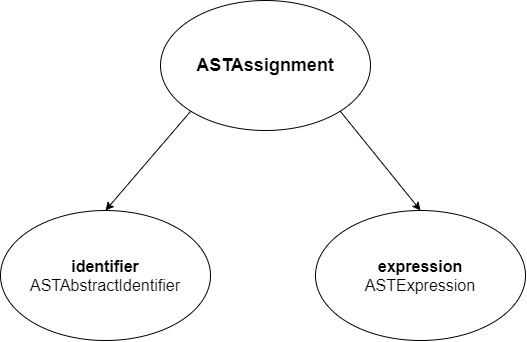
\includegraphics[width=0.55\textwidth]{astassignment2.png}
			  			\caption{ASTAssignment node}
			  			\label{fig:astassignment}
					\end{figure}
					
						\subsubsection{ASTFormalParam.java}
					
					This is a class which was created in part 1 of this assignment to represent a formal parameter. Now, it has been changed so that its member variable which represents the \textbf{identifier} is changed to be of the type of ASTAbstractIdentifier instead of ASTIdentifier so that it would support both an ASTIdentifier and an ASTArrayIdentifier
					
					\begin{figure}[H]
					\centering
			 			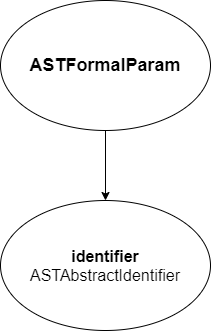
\includegraphics[width=0.25\textwidth]{astformalparam2.png}
			  			\caption{ASTFormalParam node}
			  			\label{fig:astformalparam}
					\end{figure}
					
				\subsubsection{ASTCharacterLiteral}
				
				This class was added to the other AST classes. This class extends the \textbf{ASTExpression} class and represents a char literal. This class contains only one member variable name \textbf{value} and a constructor.
				
				\begin{figure}[H]
					\centering
			 			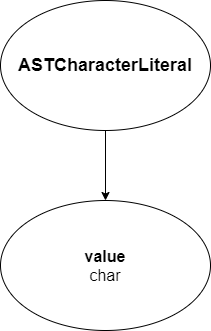
\includegraphics[width=0.25\textwidth]{ASTCharLiteral.png}
			  			\caption{ASTCharacterLiteral node}
			  			\label{fig:astcharlit}
					\end{figure}
					
									\subsubsection{Parser.java}
				
				This is the class in which one can find methods for parsing the input program. Below contains all the list of of new methods and  methods that were changed and how:
				
				\begin{enumerate}
				
				\item \textbf{literal()}: This function checks the current token and returns an AST node according to its type. In order to cater for the new feature to allow for character literals, a new switch case was added to this method to return an ASTCharacterLiteral node if the type of the token is CHARATCER\_LITERAL.
				
								\item \textbf{arraySizeIndex()}: This function is used to parse an array size or index. The EBNF rule for this is defined as \textbf{`[` \textless EXPRESSION\textgreater `]'}, hence, this function first absorbs a token of the type SQUARE\_OPEN, then gets the expression and finally, absorbs a SQUARE\_CLOSE token before returning the expression obtained.
								
				\item \textbf{arrayIdentifier(ASTIdentifier)}: This function is used to parse an array identifier. The EBNF rule for this is defined as \textbf{\textless IDENTIFIER\textgreater \textless ARRAYSIZEINDEX\textgreater}. Moreover, this function accepts an ASTIdentifier as a parameter. The function first gets the expression by calling arraySizeIndex() and then returns a new ASTArrayIdentifier node by passing the identifier passed as a parameter and the expression obtained.
				
\item \textbf{factor()}: This function is used to parse a factor. This was created in part 1 of the assignment but was changed in order to cater for character literals and arrays functionalities. This was done by adding a a case to the switch where the type of the token is checked. If the type is of type CHARACTER\_LITERAL, the function literal() is called. To cater for array identifiers, the case for when the token type is an identifier was modified by checking if the token after the identifier is of type SQUARE\_OPEN, because if so, it must mean that it is an array identifier. In fact, if this is the case the function arrayIdentifier() explained above, is called.
		
	\item \textbf{arrayValue()}: This function was created to parse an array value which may be used when declaring an array. The EBNF rules defines this as \textbf{'\{' \textless EXPRESSION\textgreater \{ ',' \textless EXPRESSION\textgreater \} '\}'}. In order to follow this rule, this function starts by defining an arraylist of expressions of type ASTExpression to hold values in it. After this, a \{' token is absorbed and the first expression is obtained and added to the array list. After this, there is a loop which goes on until as long as there are more commas to be parsed. Inside this loop, a new expression is obtained and added to the list of values. 
	
	\begin{figure}[H]
					\centering
			 			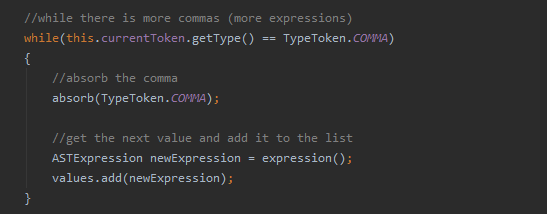
\includegraphics[width=0.55\textwidth]{astarrayvaluewhile.png}
			  			\caption{While loop in method}
			  			\label{fig:astassignment}
					\end{figure}
					
	After all the values are obtained by not finding any more commas, a `\}' token is absorbed and a new ASTArrayValue node is returned with the values found.
	

				\item \textbf{assignment()}: This function is used to parse an assignment and it was changed in order to also support an array identifier to be assigned. This was done by creating two new node explained above named \textbf{ASTAbstractIdentifier} and \textbf{ASTArrayIdentifier}. Rather than only calling identifier() and using only an ASTIdentifier, now this function makes use of an ASTAbstractIdentifier object to hold the identifier so that both an ASTIdentifier and an ASTArrayIdentifier could be held. Moroever, this method changed to first call identifier() and store this in the variable holding the identifier and then checking if there is a `[` token after the identifier which indicates that it is an array identifier. If this is the case, the identifier is passed as a parameter to the call made to the arrayIdentifier() method to obtain the arrayIdentifier. Finally, a new ASTAssignment node is created, this time with the new ASTAbstractIdentifier.
				
								\item \textbf{declaration()}: Since a new ASTDecl class was created in order to represent both a variable declaration and an array declaration, this function was created as an entry point to the functions variableDeclaration(ASTIdentifier) and arrayDeclaration(ASTIdentifier). In fact, this is confirmed by the newly created EBNF rule to define a declaration which is defined as \textbf{\textless VARIABLEDECL\textgreater | \textless ARRAYDECL\textgreater}. This function first checks if there is a LET token and if not an empty ASTDecl node is returned, as may happen in a for loop with no declaration. Otherwise, the LET token is absorbed, the identifier is obtained by calling identifier() and then it is checked if the next token is of type SQUARE\_OPEN. If it is, it means that it is an array declaration hence a call to the arrayDeclaration() method is done with the identifier passed as parameter. Otherwise, a call to the variableDeclaration() method is done with the identifier passed as a parameter.
							
				\item \textbf{variableDeclaration(ASTIdentifier)}: This function is used to parse a variable declaration and it was changed by adding an the identifier as a parameter rather than obtaining it in the function itself. This is done since the function declaration(), explained above, will be called first and then this function is called from it.
				
				\item \textbf{arrayDeclaration(ASTIdentifier)}: This function was created to parse an array declaration and it takes in an identifier as a parameter. The EBNF rule for an array declaration is defined as \textbf{'let' \textless IDENTIFIER\textgreater \textless ARRAYINDEX\textgreater ':' \textless TYPE\textgreater [ '=' \textless ARRAYVALUE\textgreater ]}. The LET token and the identifier are obtained by the declaration() function explained above which initiates this function. Then to continue following the rule, this function gets the array's size by calling arraySizeIndex(), then absorbs the COLON token, gets and sets the type to the identifier and absorbs the TYPE token. Then, it is checked if there is a value by checking if the next token is of type `='. If there is, it is absorbed and the value is obtained by calling arrayValue(). Otherwise, the ASTArrayValue node is left empty. Finally, a new ASTArrayDeclaration node is returned with the identifier and the value nodes.
				
				\item \textbf{formalParam()}: This function is used to parse a formal parameter and it was updated to match its update EBNF rule which is defined as \textbf{( \textgreater IDENTIFIER\textgreater | \textgreater ARRAYIDENTIFIER\textgreater )  [ '[' ']' ] ':' \textgreater TYPE\textgreater}. This function now starts by getting the identifier and storing it into an ASTAbstractIdentifier object since it can be both a normal identifier and an array identifier. Then, it is checked if the next token is of type SQUARE\_OPEN, because if it is, it means that the formal parameter is an array. If so, `[` and `]' tokens are 
							absorbed. After that, as used to happen before, a COLON token is absorbed and the type is obtained and set to the identifier. Finally, a new ASTFormalParam node is returned with the identifier of type ASTAbstractIdentifier.
							
		
					\item \textbf{statement()}: This function is used to parse a statement and it was updated to be able to parse an array declaration. This was done by calling the newly created declaration() function instead of variableDeclaration() in the case of a LET token. Then, as explained above, the declaration() function would decide whether to call variableDeclaration() or arrayDeclaration() itself.
				
			
				\end{enumerate}
				
				
				\subsection{Unrequired Changes}
				
				The following contains explanation to simple changes made to the visitor classes for completion. It is important to note that these changes were not required in the assignment specification and were only done for completion of the visitor classes.
				
				\subsubsection{Visitor.java}
				
				This interface was changed to include all visit methods for newly created AST classes.
				
				\subsubsection{VisitorXMLGenerator.java}
				
				In this class the visit methods for \textbf{ASTCharacterLiteral, ASTArrayValue, ASTArrayDecl, ASTDecl} and \textbf{ASTArrayIdentifier} were added for completion. The visit method for the ASTDecl class was implemented to just cater for when the declaration is empty for the case of for loops with no declaration as this was changed from the parser to return an empty ASTDecl class rather than an empty ASTVariableDecl class. Moreover, the visit method for an ASTArrayIdentifier class was also implemented since it was easy and similar to the one of a variableDeclaration. It is important to note that some other changes had to be performed since some of the ASTClasses member variables' types changed and hence some variables used in this class had to be updated, such as ASTIdentifer to ASTAbstractIdentifier and ASTVariableDeclaration to ASTDecl.
				
				\subsubsection{VisitorSemanticAnalysis.java}
				
				In this class the visit methods for \textbf{ASTCharacterLiteral, ASTArrayValue, ASTArrayDecl, ASTDecl} and \textbf{ASTArrayIdentifier} were added for completion but were not implemented. It is important to note that some other changes had to be performed since some of the ASTClasses member variables' types changed and hence some variables' types used in this class had to be updated, such as ASTIdentifer to ASTAbstractIdentifier and ASTVariableDeclaration to ASTDecl.
				
								\subsubsection{VisitorInterpreter.java}
				
				Similarly, In this class the visit methods for \textbf{ASTCharacterLiteral, ASTArrayValue, ASTArrayDecl, ASTDecl} and \textbf{ASTArrayIdentifier} were added for completion but were not implemented. Moreover, some other changes had to be performed since some of the ASTClasses member variables' types changed and hence some variables' types used in this class had to be updated, such as ASTIdentifer to ASTAbstractIdentifier and ASTVariableDeclaration to ASTDecl.
				
				\subsection{Testing}
				
				In order to test my updated versions of the lexer and parser so that they can cater for the SmallLangV2 syntax, I continued to add to the tests I had prepared for part 1 of the assignment as can be seen below.
				
				\subsubsection{Lexer testing}
				
				In order to test my changes to the lexer, I added 3 new tests to test a character declaration, an array declaration and an array assignment. Moreover, I changed my input file for the function call test by adding an extra array formal parameter. These tests are performed by preparing a list of expected tokens and then this is compared to the list of tokens returned by the lexer and the test passes or fails whether the two lists would be exactly equal to each other.
				
				\subsubsection{Parser testing}
				
				On the other hand to test the changes to the parser, I had to create the following classes.
				
				\begin{enumerate}
				\item \textbf{VisitorChecker.java} : This is a visitor class which extends the Visitor interface. This was created in order to test each node in the resultant AST tree produced by the parser. This class contains these two member variables:
				\begin{itemize}
				\item \textbf{sum}: This is a variable of type int which is used to hold the running sum.
				\item \textbf{visitedIndexes}: This is an arraylist of type Integer which holds all the visited indexes which represents nodes.
				\end{itemize}
				
				This works by having a visit method for each AST class and each node contains a unique index. Every time a node is visited, its index is added to the running sum and is inserted to the list containing the visited indexes. Obviously in each visitor method, the sub-nodes of that node are also visited.
				
				\item \textbf{ParserTest.java} : This is a test class which tests new input program snippets which I created. These snippets were made sure to target all new target features. In fact, these include an array assignment, an correct array declaration, an incorrect array declaration, an array declaration with no initialisation, array as a formal parameter a character declaration and an array assignment. This works by first parsing the input program, then the VisitorChecker class mentioned above is used by making it visit all the nodes of the tree returned by the parser. Finally, the sum member variable and the size of the visited indexes arraylist of the VisitorChecker instance are asserted.
		
				
				
				
				\end{enumerate}
				
				
				The input programs for the lexer and parser test can be found in the resources folder as can be seen i the image below.
				
					\begin{figure}[H]
					\centering
			 			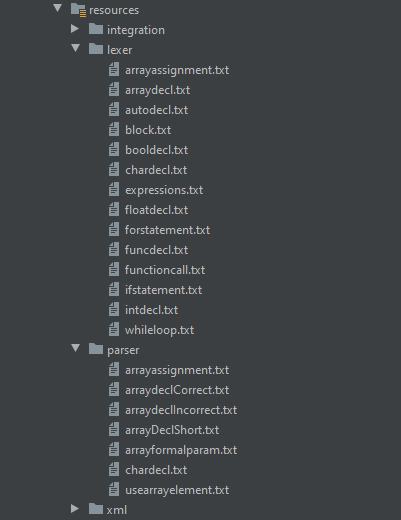
\includegraphics[width=0.55\textwidth]{filestestingpart2.png}
			  			\caption{File Structure for input programs used for testing}
			  			\label{fig:filestructure}
					\end{figure}
				
				
				
		
		\bibliographystyle{ieeetr}
		\nocite{*}
\bibliography{references2}
			
		
			
					
			\end{document}